% This is samplepaper.tex, a sample chapter demonstrating the
% LLNCS macro package for Springer Computer Science proceedings;
% Version 2.20 of 2017/10/04
%
\documentclass[runningheads]{llncs}
%
\usepackage{graphicx}
% Used for displaying a sample figure. If possible, figure files should
% be included in EPS format.
%
% If you use the hyperref package, please uncomment the following line
% to display URLs in blue roman font according to Springer's eBook style:
% \renewcommand\UrlFont{\color{blue}\rmfamily}

\begin{document}
%
\title{Contribution Title}%TODO insert super cool title here
%
\titlerunning{Abbreviated paper title}%TODO insert super cool abbrivated title here
% If the paper title is too long for the running head, you can set
% an abbreviated paper title here
%
%TODO Alternative mit Matrikelnummer? Oder so lassen?
%\author{Lukas Bl{\"u}baum\orcidID{0000-1111-2222-3333} 
%\and
%Nick D{\"u}sterhus\orcidID{1111-2222-3333-4444}
%\and
%Monika Werner\orcidID{7000575}}
\author{Lukas Bl{\"u}baum
	\and
Nick D{\"u}sterhus
 \and
Monika Werner}
%
\authorrunning{L. Bl{\"u}baum et al.}
% First names are abbreviated in the running head.
% If there are more than two authors, 'et al.' is used.
%
\institute{University of Paderborn, Padeborn 33098, Germany 
%\email{lncs@springer.com}\\
%\url{http://www.springer.com/gp/computer-science/lncs} \and
% ABC Institute, Rupert-Karls-University Heidelberg, Heidelberg, Germany\\
%\email{\{abc,lncs\}@uni-heidelberg.de}
}
%
\maketitle              % typeset the header of the contribution
%
\begin{abstract}
The goal was to create a software that is able to extract information from a Wikipedia dump and represent the information in a knowledge graph. In order to achieve this, our software uses the given systems and frameworks in each step of the process to make the resulting graph as accurate and complete as possible. 

\keywords{Knowledge Graphs  \and Semantic Web.}
\end{abstract}
%
%TODO soll code auch rein? Wuerde Seitenzahl verbessern aber die haben auch so Zugriff auf den Code und es könnte zu aehnlich zur Prasenation sein. Falls Einfügen, was, wieviel und wo? 
% TODO Seitenzahl erhoehen, soll 8 bis 10 ohne Referenzen sein
%TODO Rechtschreibfehler beheben!!!
%TODO fehlen Kapitel? 
%TODO die Schwierigkeitseinschaetzungen sind komplett geraten
%TODO am Ende: alle Spuren des sample texts entfernen, waren nur als template drin behalten worden
%TODO bearbeitete TODOs entfernen, sobald sie bearbeitet wurden.
%
\section{The Task}
The task given to us was to create a programm that can create a knowledge graph, agraph that represents entities as nodes and relations between those entities as edges, from a large text corpus, in this case a Wikipedia dump, in order to learn the basics of Semantic Web technologies. We should learn how to extract, aggregate and present information in scalable ways. To facilitate this task we were introduced to several tools including FOX and DBpedia Spotlight which are capable of handling parts of the task on their own. To show how well our programm works, its results were compared to the results from DBpedia. 
\section{The Process}
There are several steps that need to be taken in order to create a knowledge graph from a given text which will be demonstrated on the following small example text: 
\begin{example} Obama was born on August 4, 1961, at Kapiolani Medical Center for Women and Children in Honolulu, Hawaii. He graduated from Havard University.\end{example}
\subsection{Preprocessing}
\subsubsection{Extraction and Cleaning of the Text from a Wikipedia Dump}
The Wikipedia dumps that the software works on come as plaintexts without markup, infoboxes or chapter subdivison but they still contain elements that are undesired for later steps in the process. Such elements include unnecessary URLs, paranthesis, whitespace, nullchar and certain symbols. In order to get rid of these unwanted elements, we created a class called WikiCleaner that reads through the dump, recognizes the unwanted elements, removes them and writes the resulting text into an output file for usage in later steps. The result is a simple text containing only the letters from the English alphabet, numbers, periods and of course simple spaces.  

In order to speed up the cleaning process, the WikiCleaner uses Reader and Writer threads for reading the input file and writing the output file respectivly. 

This step was the easiest part of the entire process and uses only standard Java libraries. There were no difficulties during the implemention of this step. 

\subsubsection{Coreference Resolution}
Another step that needs to be taken before the information can be properly extracted is replacing all the pronouns with the corresponding noun it refers to. This is done so that the process can find all he information it needs in the current sentence and doesn't have to look back on previous parts of the text in order to understand the pronouns. 

% TODO replace x with proper reference in proper style
% TODO how is the last matching entity found? Going back in text or saved in variables, one for male one for female and one for genderless entities?
For this task we use the Stanford CoreNLP in order to split the text into tokens (roughly "words", see x) an check each token whether it is a pronoun or not. If it is a pronoun, we replace it with the last mentioned noun that matches its grammatical gender.

After both steps of te preprocessing are done, our text example looks as follows:
\begin{example} Obama was born on August 4 , 1961 , at Kapiolani Medical Center for Women and Children in Honolulu , Hawaii . Obama graduated from Havard University. \end{example}

This is still a relative easy part after unerstanding and learning how to use Stanford NLP properly.

\subsection{Named Entity Recognition}
In this part of the process we scan through the cleaned text to identify named entities like people, locations etc. which will be the nodes of our graph later on. 

For this step we use the DBpedia Spotlight web service. We send the cleaned text to DBpedia Spotlight and receive a JSON response.The response is then parsed and the found entities and their information is stored in objects of our Entity class.

From our example text, the word that are recognized as named entitis are those that are underlined in the following:

\begin{example}\underline{Obama} was born on August 4, 1961, at \underline{Kapiolani} Medical Center for Women and Children in \underline{Honolulu}, \underline{Hawaii}. \underline{Obama} graduated from \underline{Havard University} .\end{example}

As the process of entity recognition is mainly done by DBpedia Spotlight our main task in this step is simply to send the data and deal with the response. Therefore, implementing this step was a bit more demanding then the imlementation of the first but still not particuary difficult.

\subsection{Entity Disambiguation}

After finding the named entities we need to recognize which entities are actually refered to by the named entities found in the Wikipedia article. There are many people, places etc. sharing the same or similar names so we need to find out which entity was ment by the article in order to build the correct relations between them later on.

This step is partially already done with DBpedia Spotlight, however, in addition to it we also use FOX. Again, we simply sent our data and parse and save the response for later steps. 

As this is completely done by the given frameworks, we did not have to add much.

\subsection{Relation Extraction}

After recognizing the entities correctly we need to find the relations between them mentioned in the given Wikipedia dump to finish our knowledge graph. The relation become the edges of the graph.

The type of relation we are most interested in are binary relations, so relations between only two entities an not more. Therefore, we need to find those first. The relations of this type that can be found in our example include:
\begin{example}
First sentence: Obama - be bear on - August 4 1961. (among others)

Second sentence: Obama - graduate from - Havard Law school (among others)\end{example}

Afterwards, we add the relation to our graph. In order to do so, we first look at the subject of the binary relation. In both sentences from our example we recognize "Obama" as the subject with its type including "Person". Then we look at the object of the relation. In the first sentence, we detect that the object contains numbers, which can indicate that the object contains either a date or a number literal. We check whether the object is a date and if it is not, we extract it as a single literal of a fitting number type if it is a number or keep it as a string if the number just happens to be part of a name and therefore not convertable to any other type of literal. In our case, we detect "August" is a month and therefore convert the whole object to the proper dateformat 1961-08-04. In the second sentence, we detect "Hardvard University" as another entity of type EducationalInstitution. Then, in order to be able to map the found relation to the correct property, we look at the predicate of the sentences and check for keywords. In our first sentence, we find "bear" in a relation with "Person" as the domain and xsd:date as range so we search for a property which fits this keyword, domain and range and get dbo:birthDate, while in our second sentence we find the keyword "graduate" with "Person" as domain and " EducationalInstitution" as range and get dbo:almaMater as the fitting property. With these informations, we turned the first and second sentence of our example into the following triples:
\begin{example} First sentence: dbo:Barack\_Obama dbo:birhtDate "1961-08-04".
	
	Second sentence: dbo:Barack\_Obama dbo:almaMater dbo:Havard\_University.\end{example}

These triples can now be properly added to our knowledge graph. After this has been done with all found triples our knowledge graph from the given text is as far completed as the programm is capable to do so.

For this step again we use FOX and Spotlight. We use FOX in "re" mode for entity recognition and relation extraction, however FOX does not recognize many triples and misses too many relations. Therefore we implemented our own method using Spotlight and OpenIE.
We use DBdia Spotlight first for named entity recognition so that we can run our method concurrent to FOX. 

\section{Correctness and Runtime}
%TODO Benchmarks!!Testresults!!



%\subsubsection{Sample Heading (Third Level)} Only two levels of
%headings should be numbered. Lower level headings remain unnumbered;
%they are formatted as run-in headings.

%\paragraph{Sample Heading (Fourth Level)}
%The contribution should contain no more than four levels of
%headings. Table~\ref{tab1} gives a summary of all heading levels.

%\begin{table}
%\caption{Table captions should be placed above the
%tables.}\label{tab1}
%\begin{tabular}{|l|l|l|}
%\hline
%Heading level &  Example & Font size and style\\
%\hline
%Title (centered) &  {\Large\bfseries Lecture Notes} & 14 point, bold\\
%1st-level heading &  {\large\bfseries 1 Introduction} & 12 point, bold\\
%2nd-level heading & {\bfseries 2.1 Printing Area} & 10 point, bold\\
%3rd-level heading & {\bfseries Run-in Heading in Bold.} Text follows & 10 point, bold\\
%4th-level heading & {\itshape Lowest Level Heading.} Text follows & 10 point, italic\\
%\hline
%\end{tabular}
%\end{table}


%\noindent Displayed equations are centered and set on a separate
%line.
%\begin{equation}
%x + y = z
%\end{equation}
%Please try to avoid rasterized images for line-art diagrams and
%schemas. Whenever possible, use vector graphics instead (see
%Fig.~\ref{fig1}).

%\begin{figure}
%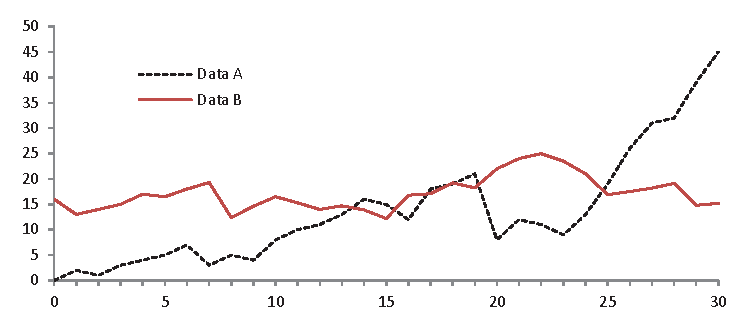
\includegraphics[width=\textwidth]{fig1.eps}
%\caption{A figure caption is always placed below the illustration.
%Please note that short captions are centered, while long ones are
%justified by the macro package automatically.} \label{fig1}
%\end{figure}

%\begin{theorem}
%This is a sample theorem. The run-in heading is set in bold, while
%the following text appears in italics. Definitions, lemmas,
%propositions, and corollaries are styled the same way.
%\end{theorem}
%
% the environments 'definition', 'lemma', 'proposition', 'corollary',
% 'remark', and 'example' are defined in the LLNCS documentclass as well.
%
%\begin{proof}
%Proofs, examples, and remarks have the initial word in italics,
%while the following text appears in normal font.
%\end{proof}
%For citations of references, we prefer the use of square brackets
%and consecutive numbers. Citations using labels or the author/year
%convention are also acceptable. The following bibliography provides
%a sample reference list with entries for journal
%articles~\cite{ref_article1}, an LNCS chapter~\cite{ref_lncs1}, a
%book~\cite{ref_book1}, proceedings without editors~\cite{ref_proc1},
%and a homepage~\cite{ref_url1}. Multiple citations are grouped
%\cite{ref_article1,ref_lncs1,ref_book1},
%\cite{ref_article1,ref_book1,ref_proc1,ref_url1}.
%
% ---- Bibliography ----
%
% BibTeX users should specify bibliography style 'splncs04'.
% References will then be sorted and formatted in the correct style.
%
% \bibliographystyle{splncs04}
% \bibliography{mybibliography}
%
\begin{thebibliography}{8} %TODO echte Referenzen
\bibitem{ref_article1}
Author, F.: Article title. Journal \textbf{2}(5), 99--110 (2016)

\bibitem{ref_lncs1}
Author, F., Author, S.: Title of a proceedings paper. In: Editor,
F., Editor, S. (eds.) CONFERENCE 2016, LNCS, vol. 9999, pp. 1--13.
Springer, Heidelberg (2016). \doi{10.10007/1234567890}

\bibitem{ref_book1}
Author, F., Author, S., Author, T.: Book title. 2nd edn. Publisher,
Location (1999)

\bibitem{ref_proc1}
Author, A.-B.: Contribution title. In: 9th International Proceedings
on Proceedings, pp. 1--2. Publisher, Location (2010)

\bibitem{ref_url1}
LNCS Homepage, \url{http://www.springer.com/lncs}. Last accessed 4
Oct 2017
\end{thebibliography}
\end{document}
